Multi-task learning (MTL) is an important machine learning paradigm that
aims at improving the generalization performance of a task using other related
tasks. 
Such framework has been widely studied by
\newcite{thrun96,caruana97,evgeniou04,ando05,argyriou07,kumar12}, among many
others. In the context of deep neural networks, MTL has
been applied successfully to various problems ranging from language
\cite{liu15}, to vision
\cite{donahue14},
and speech \cite{heigold13,huang2013cross}.

Recently, sequence to sequence (\ssl{}) learning
\cite{kal13,sutskever14,cho14} emerges as an effective paradigm for dealing with
variable-length inputs and outputs. \ssl{} learning, at its core, uses
recurrent neural networks to map variable-length input sequences to
variable-length output sequences.  While relatively new, the \ssl{}
approach has achieved state-of-the-art results in not only its original
application -- machine translation --
\cite{luong15,jean15,luong15attn,jean15wmt,luong15iwslt}, but also image caption generation \cite{vinyals15caption},
and constituency parsing \cite{vinyals15grammar}. 

Despite the popularity of multi-task learning and sequence to sequence
learning, there has been little work in combining MTL with \ssl{}
learning. To the best of our knowledge, there is only one recent
publication by \newcite{dong15} which applies a \ssl{} models for machine
translation, where the goal is to translate from one language to
multiple languages.
In this work, we propose three MTL
approaches that complement one another: (a) the {\it \otm} approach -- for
tasks that can have an encoder in common, such as translation and parsing; this 
applies to the multi-target translation setting in \cite{dong15} as well, (b)
the {\it \mto} approach -- useful for multi-source
translation or tasks in which only the decoder can be easily shared,
such as translation and image captioning, and lastly, (c) the {\it \mtm} approach -- which share
multiple encoders and decoders through which we study the effect of unsupervised
learning in translation.
We show
that syntactic parsing and image caption generation improves the
translation quality between English and German by up to +$1.5$ BLEU points over
strong single-task baselines on the WMT benchmarks. 
Furthermore, we have established a new {\it state-of-the-art} result in
constituent parsing with 93.0 F$_1$.
We also explore two unsupervised learning
objectives, sequence autoencoders \cite{dai15} and skip-thought vectors
\cite{kiros15skip}, and reveal their interesting properties in the MTL setting: autoencoder helps less in terms of
  perplexities but more on BLEU scores compared to skip-thought.
%Our novel findings reveal that the skip-thought objective improves
%translation while the sequence autoencoders does not.
\begin{figure}%[tbh]
\centering
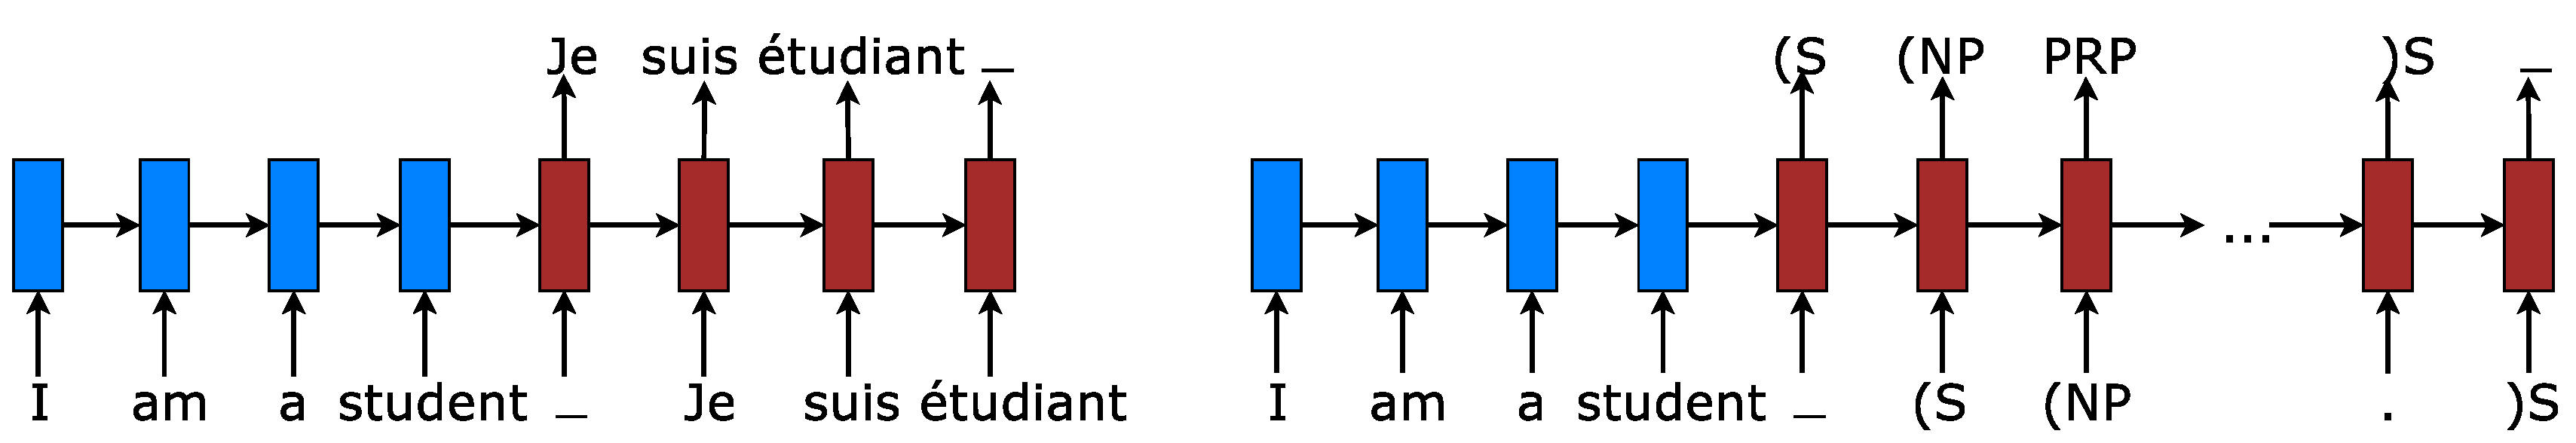
\includegraphics[width=1\textwidth, clip=true, trim= 0 0 0
0]{img/6-1_seq2seq}
\caption[Sequence to sequence learning examples]{{\bf Sequence to sequence learning examples} -- (left) machine
translation \cite{sutskever14} and ({\it right}) constituent parsing
\cite{vinyals15grammar}.}
\label{f:s2s}
\end{figure}


